\documentclass{article}

% For math environments
\usepackage{amsmath, amsfonts}
% For links
\usepackage[hidelinks]{hyperref}
% So space it put between paragraphs
\usepackage{parskip}
% For figures
\usepackage{tikz}
% Set the margins to not be ridiculous
\usepackage[margin=0.75in]{geometry}
% For multiple columns
\usepackage{multicol}
% For controlling enum/itemize spacing and indentation
\usepackage{enumitem}

% For tikz plots
\usepackage{pgfplots}
% This isn't needed but avoids a compiler warning
\pgfplotsset{compat=1.16}

% Allow multi-line equations to be broken across pages
\allowdisplaybreaks

% Use @ as a letter
\makeatletter

% Scale down all tikz coordinates while maintaining font size
\tikzset{every picture/.style={scale=0.45, every picture/.style={}}}


% Macros
% Monospace code
\def\code#1{\texttt{#1}}

% Greek letters
\def\a{\alpha}
\def\b{\beta}
\def\g{\gamma}
\def\d{\delta}
\def\D{\Delta}

% Some common sets
\def\es{\varnothing}
\def\ints{{\mathbb{Z}}}

% Commands that make life easier
\newcommand\gath[1]{\begin{gather} #1 \end{gather}}
\newcommand\gaths[1]{\begin{gather*} #1 \end{gather*}}
\newcommand\ali[1]{\begin{align} #1 \end{align}}
\newcommand\parens[1]{\left( #1 \right)}
\newcommand\squares[1]{\left[ #1 \right]}
\newcommand\braces[1]{\left\{ #1 \right\}}
\newcommand\angles[1]{\left\langle #1 \right\rangle}
\newcommand\deriv[2]{\frac{d #1}{d #2}}
\newcommand\abs[1]{\left| #1 \right|}
\newcommand\floor[1]{\left\lfloor #1 \right\rfloor}
\newcommand\ceil[1]{\left\lceil #1 \right\rceil}
\DeclareMathOperator{\lcm}{lcm}
\def\non{\nonumber \\}
\newcommand\unit[1]{~\mathrm{#1}}
\newcommand\combos[2]{{}_{#1}C_{#2}}

% Set stuff
\def\ss{\subseteq}

% Multiline equation space
\def\mlesp{\hspace{1.2cm}}

% For grid diagrams
\newcommand\gridbox[3]{\draw (#1,#2) rectangle (#1+1,#2+1) node[pos=.5] {#3};}
\newcommand\gridboxh[3]{\draw[fill=red!20] (#1,#2) rectangle (#1+1,#2+1) node[pos=.5] {#3};}
\newcommand\gridboxb[3]{\draw[fill=black] (#1,#2) rectangle (#1+1,#2+1) node[pos=.5] {#3};}
\newcommand\gridsym[3]{\node at (#1+0.5,#2+0.5) {$#3$};}
\newcommand\gridblank[2]{\filldraw[draw=gray, color=gray] (#1,#2) rectangle (#1+1,#2+1);}
\newcommand\gridcirc[2]{\draw (#1 + 0.5,#2 + 0.5) circle (0.25);}
\newcommand\cwlab[3]{
  \def\dd{0.15}
  \draw (#1 + \dd - 0.03, #2 + 1 - \dd) node {\scriptsize #3};
}

\def\bbw{3.5}
\def\bbh{2}
\newcommand\bigbox[3]{\draw (#1*\bbw,#2*\bbh) rectangle (#1*\bbw+\bbw,#2*\bbh+\bbh) node[pos=.5] {#3};}
\newcommand\bbtextr[3]{\node[right] at (#1*\bbw,#2*\bbh+0.5*\bbh) {#3};}
\newcommand\bbtextb[3]{\node[align=center] at (#1*\bbw+0.5*\bbw,#2*\bbh+0.5*\bbh) {#3};}

% Box puzzle stock answer
\newcommand\boxans[1]{
  Logic was used to deduce the solution:

  #1

  This was verified using Python as well as shown to be unique with a brute force approach.
}

% Standard crossnumber grid
\newcommand\crossnumstd[9]{
  \begin{center}
    \begin{tikzpicture}[scale=2]
      \gridbox{0}{2}{#1}
      \gridbox{1}{2}{#2}
      \gridbox{2}{2}{#3}
      \gridbox{0}{1}{#4}
      \gridbox{1}{1}{#5}
      \gridbox{2}{1}{#6}
      \gridbox{0}{0}{#7}
      \gridbox{1}{0}{#8}
      \gridbox{2}{0}{#9}

      % Labels
      \cwlab{0}{2}{1}
      \cwlab{1}{2}{2}
      \cwlab{2}{2}{3}
      \cwlab{0}{1}{4}
      \cwlab{0}{0}{5}
    \end{tikzpicture}
  \end{center}
}

% Multiple numbers
\newcommand\mn[1]{$#1$'s}

% Commands for problems
\newcommand\problem[4]{
\section*{#1}

\textbf{Question:} #3

\textbf{Answer:} #2

\textbf{Explanation:} #4
}
\newcommand\aproblem[4]{\problem{Dec #1}{#2}{#3}{#4}}
\newcommand\cproblem[4]{\problem{Problem #1}{#2}{#3}{#4}}

\newcommand\xref@advent[2]{#1 Advent, Dec~#2 problem}
\newcommand\xref@card[2]{#1 Christmas Card, Problem #2}

% For answered verified with Python
\newcommand{\verified}{This was verified with a brute-force Python program.}

\def\advent@xxi@i{
  The geometric mean of a set of $n$ numbers can be computed by multiplying together all the numbers then computing the $n$th root of the result.

  The factors of $4$ are $1$, $2$ and $4$. The geometric mean of these is 2.

  The factors of $6$ are $1$, $2$, $3$, and $6$. The geometric mean of these is $\sqrt{6}$.

  The geometric mean of all the factors of today's number is $22$.
}

\def\advent@xxi@ii{
  The number $7n$ has $37$ factors (including $1$ and the number itself).
  How many factors does $8n$ have?
}

\def\advent@xxi@iii{
  If you write out the numbers from $1$ to $1000$ (inclusive), how many times will you write the digit $0$?
}

\def\advent@xxi@iv{
  Put the digits $1$ to $9$ (using each digit exactly once) in the boxes so that the sums are correct.
  The sums should be read left to right and top to bottom ignoring the usual order of operations.
  For example, $4 + 3 \times 2$ is $14$, not $10$.
  Today's number is the product of the numbers in the red boxes.

  \grid@advent@xxi@iv{}{}{}{}{}{}{}{}{}
}

\def\advent@xxi@v{
  How many different isosceles triangles are there whose perimeter is $50$ units, and whose area is an integer number of units squared?

  (Two triangles that are rotations, reflections and translations of each other are counted as the same triangle. Triangles with an area of 0 should not be counted.)
}

\def\advent@xxi@vi{
  When $12345$ is divided by today's number, the remainder is $205$.
  When $6789$ is divided by today's number, the remainder is $112$.
}

\newcommand\dec@ai{0.30901699437494745}
\newcommand\dec@aii{0.8090169943749475}
\newcommand\dec@bi{0.5877852522924731}
\newcommand\dec@bii{0.9510565162951535}
\newcommand\decagon[5]{
  \def\ai{\dec@ai*#3+#1}
  \def\aii{\dec@aii*#3+#1}
  \def\bi{\dec@bi*#3+#2}
  \def\bii{\dec@bii*#3+#2}
  \draw (#3+#1, #2) -- (\aii, \bi) -- (\ai, \bii) -- (-\ai, \bii) -- (-\aii, \bi) -- (-#3+#1, #2) -- (-\aii, -\bi) -- (-\ai, -\bii) -- (\ai, -\bii) -- (\aii, -\bi) -- cycle;
  \fill[fill=red] (-\ai, -\bii) -- (#4*#3+#1, #5*#3+#2) -- (\ai, -\bii) -- cycle;
}
\def\advent@xxi@vii{
  The picture below shows eight regular decagons.
  In each decagon, a red triangle has been drawn with vertices at three of the vertices of the decagon.

  \begin{center}
    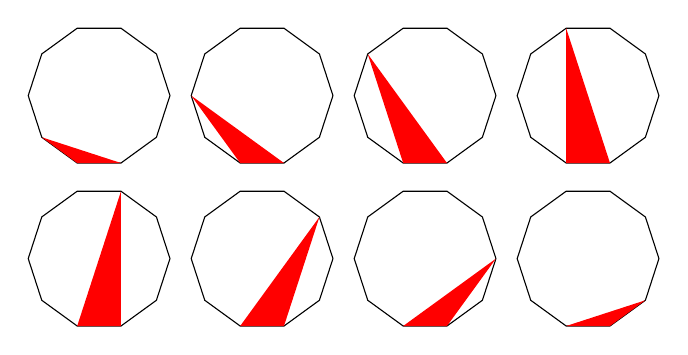
\begin{tikzpicture}
      \def\dr{2}
      \def\spc{2.3*\dr}

      \decagon{0*\spc}{\spc}{\dr}{-\dec@aii}{-\dec@bi}
      \decagon{1*\spc}{\spc}{\dr}{-1}{0}
      \decagon{2*\spc}{\spc}{\dr}{-\dec@aii}{\dec@bi}
      \decagon{3*\spc}{\spc}{\dr}{-\dec@ai}{\dec@bii}

      \decagon{0*\spc}{0}{\dr}{\dec@ai}{\dec@bii}
      \decagon{1*\spc}{0}{\dr}{\dec@aii}{\dec@bi}
      \decagon{2*\spc}{0}{\dr}{1}{0}
      \decagon{3*\spc}{0}{\dr}{\dec@aii}{-\dec@bi}
    \end{tikzpicture}
  \end{center}

  The area of each decagon is $240$.
  What is the total area of all the red triangles?
}

\def\advent@xxi@viii{
  The sum of three integers is $51$.
  The product of the same three integers is $836$. What is the product of largest integer and the second-largest integer?
}

\def\advent@xxi@ix{
  Eve writes down a sequence of consecutive positive integers (she writes more than one number).
  The sum of the numbers Eve has written down is $844$.
  Today's number is the smallest integer that Eve has written down.
}

\def\advent@xxi@x{
  Put the digits $1$ to $9$ (using each digit exactly once) in the boxes so that the sums are correct.
  Today's number is the largest number you can make using the digits in the red boxes.

  \grid@advent@xxi@x{}{}{}{}{}{}{}{}{}
}

\def\advent@xxi@xi{
  The integers are written in a triangle as shown below:
  \begin{center}
    \begin{tabular}{ccccccc}
         &    &    & 1    &    &    &    \\
         &    & 2  & 3    & 4  &    &    \\
         & 5  & 6  & 7    & 8  & 9  &    \\
      10 & 11 & 12 & 13   & 14 & 15 & 16 \\
         &    &    & etc. &    &    &
    \end{tabular}
  \end{center}
  Today's number appears directly above the number $750$ in the triangle of integers.
}

\def\advent@xxi@abgrid{
  \begin{center}
    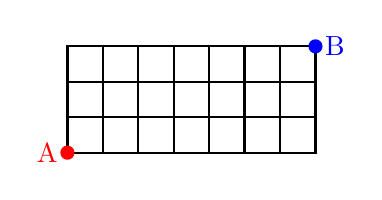
\begin{tikzpicture}
      \def\gs{1}
      % Grid
      \foreach \i in {0,...,6}{
          \foreach \j in {0,...,2}{
              \draw[thick] (\i * \gs, \j * \gs) rectangle (\i * \gs + \gs, \j * \gs + \gs);
            }
        }
      % Points
      \fill[color=red] (0, 0) circle (0.2) node[color=red,left] {A};
      \fill[color=blue] (7*\gs, 3*\gs) circle (0.2) node[color=blue,right] {B};
    \end{tikzpicture}
  \end{center}
}
\def\advent@xxi@xii{
  You start at the point marked A in the picture below. You want to get to the point marked B.
  You may travel \textbf{to the right} or \textbf{upwards} along the black lines.

  \advent@xxi@abgrid

  Today's number is the total number of possible routes to get from A to B.
}

\def\advent@xxi@xiii{
  The diagram below shows three circles and two triangles.
  The three circles all meet at one point.
  The vertices of the smaller red triangle are at the centers of the circles.
  The lines connecting the vertices of the larger blue triangle to the point where all three circles meet are diameters of the three circles.

  \begin{center}
    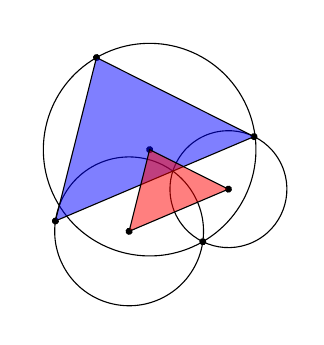
\begin{tikzpicture}[rotate=30,transform shape]
      \def\bcr{3}
      \def\scr{0.55*\bcr}
      \def\sca{34}
      \def\mcr{0.7*\bcr}
      \def\mca{142}
      \def\pr{0.1}

      % Circles
      \draw (0, \bcr) circle (\bcr);
      \draw (\sca: \scr) circle (\scr);
      \draw (\mca: \mcr) circle (\mcr);

      % Points
      \fill (0, 0) circle (\pr);
      \fill (0, \bcr) circle (\pr);
      \fill (0, 2*\bcr) circle (\pr);
      \fill (\sca: \scr) circle (\pr);
      \fill (\sca: 2*\scr) circle (\pr);
      \fill (\mca: \mcr) circle (\pr);
      \fill (\mca: 2*\mcr) circle (\pr);

      % Triangles
      \draw[fill=blue,fill opacity=0.5] (\mca: 2*\mcr) -- (0, 2*\bcr) -- (\sca: 2*\scr) -- cycle;
      \draw[fill=red,fill opacity=0.5] (\mca: \mcr) -- (0, \bcr) -- (\sca: \scr) -- cycle;
    \end{tikzpicture}
  \end{center}

  The area of the smaller red triangle is $226$.
  What is the area of the larger blue triangle?
}

\def\advent@xxi@xiv{
  You start at the point marked A in the picture below.
  You want to get to the point marked B.
  You may travel \textbf{to the right}, \textbf{upwards}, or \textbf{to the left} along the black lines, but you cannot pass along the same line segment more than once.

  \advent@xxi@abgrid

  Today's number is the total number of possible routes to get from A to B.
}

\newcommand\pyramid@advent@xxi@xvi[6]{
  \begin{center}
    \begin{tabular}{cccccc}
      (row 1) &    &    & #1   &    &    \\
      (row 2) &    & #2 &      & #3 &    \\
      (row 3) & #4 &    & #5   &    & #6 \\
              &    &    & etc. &    &
    \end{tabular}
  \end{center}
}
\def\advent@xxi@xv{
  The odd numbers are written in a pyramid.

  \pyramid@advent@xxi@xvi{1}{3}{5}{7}{9}{11}

  What is the mean of the numbers in the 19th row?
}

\newcommand\grid@advent@xxi@xvi[9]{
  \begin{center}
    \begin{tikzpicture}[scale=2]
      \gridbox{0}{2}{#1}
      \gridbox{1}{2}{#2}
      \gridbox{2}{2}{#3}
      \gridbox{0}{1}{#4}
      \gridbox{1}{1}{#5}
      \gridbox{2}{1}{#6}
      \gridbox{0}{0}{#7}
      \gridbox{1}{0}{#8}
      \gridbox{2}{0}{#9}

      % Labels
      \cwlab{0}{2}{1}
      \cwlab{1}{2}{2}
      \cwlab{2}{2}{3}
      \cwlab{0}{1}{4}
      \cwlab{0}{0}{5}
    \end{tikzpicture}
  \end{center}
}
\def\advent@xxi@xvi{
  Each clue in this crossnumber is formed of two parts connected by a logical connective: AND means that both parts are true; NAND means that at most one part is true; OR means that at least one part is true; NOR means that neither part is true; XOR means that exactly one part is true; XNOR means that either both parts are false or both parts are true.
  No number starts with $0$.

  \begin{multicols}{2}
    \grid@advent@xxi@xvi{}{}{}{}{}{}{}{}{}

    \columnbreak

    \begin{enumerate}
      \item \textbf{1A} is a palindrome XNOR \textbf{1D} is a palindrome.
      \item \textbf{1A} is greater than $350$ NOR \textbf{1D} is less than $150$.
      \item \textbf{3D} is odd NAND \textbf{4A} and \textbf{2D} are equal.
      \item \textbf{3D} is prime XOR \textbf{5A} is odd.
      \item \textbf{4A} is a cube AND \textbf{2D} is a cube.
      \item The sum of the digits of \textbf{3D} is $2$ OR the sum of the digits of \textbf{5A} is $5$.
      \item Today's number is \textbf{1D}.
    \end{enumerate}
  \end{multicols}
}

\def\advent@xxi@xvii{
  The digital product of a number is computed by multiplying together all of its digits. For example, the digital product of $6273$ is $252$.

  Today's number is the smallest number whose digital product is $252$.
}

\def\advent@xxi@xviii{
  Put the digits $1$ to $9$ (using each digit exactly once) in the boxes so that the sums are correct.
  The sums should be read left to right and top to bottom ignoring the usual order of operations.
  For example, $4 + 3 \times 2$ is $14$, not $10$.
  Today's number is the product of the numbers in the red boxes.

  \grid@advent@xxi@xviii{}{}{}{}{}{}{}{}{}
}

\def\advent@xxi@xix{
  The equation $352x^3 - 528x^2 + 90 = 0$ has three distinct real-valued solutions.

  Today's number is the number of integers $a$ such that the equation $352x^3 - 528x^2 + a = 0$ has three distinct real-valued solutions.
}

\def\advent@xxi@xx{
  What is the area of the largest area triangle that has one side of length $32$ and one side of length $19$?
}

\newcommand\grid@advent@xxi@xxi[9]{
  \begin{center}
    \begin{tikzpicture}
      \bigbox{0}{3}{#1}
      \bigbox{1}{3}{#2}
      \bigbox{2}{3}{#3}
      \bbtextr{3}{3}{\textbf{today's number}}

      \bigbox{0}{2}{#4}
      \bigbox{1}{2}{#5}
      \bigbox{2}{2}{#6}
      \bbtextr{3}{2}{prime}

      \bigbox{0}{1}{#7}
      \bigbox{1}{1}{#8}
      \bigbox{2}{1}{#9}
      \bbtextr{3}{1}{square}

      \bbtextb{0}{0}{cube}
      \bbtextb{1}{0}{odd}
      \bbtextb{2}{0}{multiple\\of $11$}
    \end{tikzpicture}
  \end{center}
}
\def\advent@xxi@xxi{
  Arrange the digits $1$–$9$ (using each digit exactly once) so that the three digit number in: the middle row is a prime number; the bottom row is a square number; the left column is a cube number; the middle column is an odd number; the right column is a multiple of $11$.
  The $3$-digit number in the first row is today's number.

  \grid@advent@xxi@xxi{}{}{}{}{}{}{}{}{}
}

\def\advent@xxi@xxii{
  There are $12$ ways of placing $2$ tokens on a $2 \times 4$ grid so that no two tokens are next to each other horizontally, vertically or diagonally:

  \begin{center}
    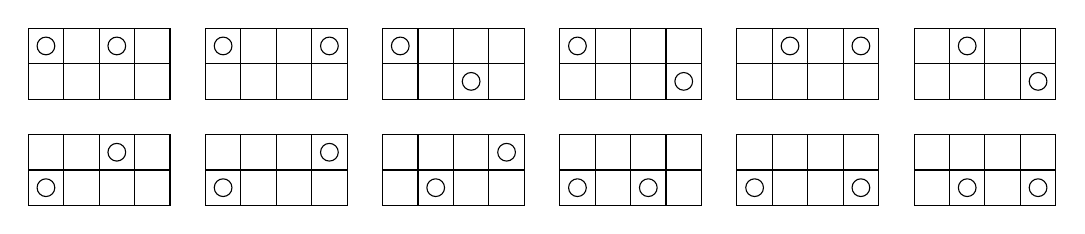
\begin{tikzpicture}
      % Draw all the grids
      \foreach \gi in {0,1}{
          \foreach \gj in {0,...,5}{
              \foreach \i in {0,1}{
                  \foreach \j in {0,...,3}{
                      \gridbox{5*\gj + \j}{3*\gi + \i}{}
                    }
                }
            }
        }

      % Place token circles
      \gridcirc{0}{4}
      \gridcirc{2}{4}
      \gridcirc{5}{4}
      \gridcirc{8}{4}
      \gridcirc{10}{4}
      \gridcirc{12}{3}
      \gridcirc{15}{4}
      \gridcirc{18}{3}
      \gridcirc{21}{4}
      \gridcirc{23}{4}
      \gridcirc{26}{4}
      \gridcirc{28}{3}
      \gridcirc{0}{0}
      \gridcirc{2}{1}
      \gridcirc{5}{0}
      \gridcirc{8}{1}
      \gridcirc{11}{0}
      \gridcirc{13}{1}
      \gridcirc{15}{0}
      \gridcirc{17}{0}
      \gridcirc{20}{0}
      \gridcirc{23}{0}
      \gridcirc{26}{0}
      \gridcirc{28}{0}
    \end{tikzpicture}
  \end{center}

  Today's number is the number of ways of placing $2$ tokens on a $2 \times 21$ grid so that no two tokens are next to each other horizontally, vertically or diagonally.
}

\def\advent@xxi@xxiii{
  I draw the parabola $y = x^2$ and mark points on the parabola at $x = 17$ and $x = -6$.
  I then draw a straight line connecting these two points.

  At which value of $y$ does this line intercept the $y$-axis?
}

\def\advent@xxi@xxiv{
  The digital product of a number is computed by multiplying together all of its digits.
  For example, the digital product of $1522$ is $20$.

  How many $12$-digit numbers are there whose digital product is $20$?
}

\def\card@xxi@i{
  What is the sum of all the odd integers between $0$ and $30$?
}

\def\card@xxi@ii{
  What is the sum of all the odd integers between $0$ and $5668$?
}

\def\card@xxi@iii{
  What is the smallest integer with a digital sum of $28$ and a digital product of $10000$?
}

\def\card@xxi@iv{
  What is the smallest integer with a digital sum of $41$ and a digital product of $432000$?
}

\def\card@xxi@v{
  What is the area of the largest area dodecagon that will fit inside a circle with area $111185 \pi$?
}

\def\card@xxi@vi{
  What is the area of the largest area heptagon that will fit inside a semicircle with area $115185 \pi$?
}

\def\card@xxi@vii{
  How many terms are there in the (simplified) expansion of $(x + y + z)^2$?
}

\def\card@xxi@viii{
  How many terms are there in the (simplified) expansion of $(x + y + z)^{41172}$?
}

\def\card@xxi@ix{
  What is the largest integer that cannot be written as $4a + 5b$ for non-negative integers $a$ and $b$?
}

\def\card@xxi@x{
  What is the largest integer that cannot be written as $83409a + 66608b$ for non-negative integers $a$ and $b$?
}

\def\card@xxi@xi{
  How many positive integers are there below $100$ whose digits are all non-zero and different?
}

\def\card@xxi@xii{
  How many positive integers are there whose digits are all non-zero and different?
}

\def\card@xxi@xiii{
  What is the only integer for which taking the geometric mean of all its factors (including $1$ and the number itself) gives $2$?
}

\def\card@xxi@xiv{
  What is the only integer for which taking the geometric mean of all its factors (including $1$ and the number itself) gives $25$?
}

\input{boxes}

\begin{document}

\title{Matthew Scroggs Advent Calendar 2025 Answers}
\author{Dan Whitman}
\date{}

\maketitle

Magic link: \href{http://mscroggs.co.uk/adventcode/5kGf6WdI}{http://mscroggs.co.uk/adventcode/5kGf6WdI}
% Answers: \href{https://www.mscroggs.co.uk/puzzles/advent2025}{https://www.mscroggs.co.uk/puzzles/advent2025}

\newcommand{\verified}{This was verified with a brute-force Python program.}

\aproblem{1}{648}{\advent@xxv@i}{
  We will approach this like a permutation.
  There are $9$ numbers for the first digit (i.e. $1$ through $9$), noting that this cannot be zero.
  There are also $9$ numbers to choose from for the second digit (i.e. $0$ through $9$ minus the one digit already chosen to be the first).
  Clearly then there are only $8$ numbers from which to choose for the final digit (i.e. $0$ through $9$ minus the two already chosen).
  Hence, there are
  \gath{
    9 \cdot 9 \cdot 8 = 648
  }
  three-digit numbers whose digits are all different.
  \verified{}
}

\aproblem{2}{192}{\advent@xxv@ii}{
  There are $9$ single digit numbers (i.e. $1$ through $9$) and $9 \cdot 10 = 90$ two-digit numbers (i.e. $10$ through $99$).
  And of course we have our single three-digit number $100$.
  Thus, if all these numbers are written down, there will be
  \gath{
    9 \cdot 1 + 90 \cdot 2 + 1 \cdot 3 = 192
  }
  total digits written.
  This was verified with a brute-force Python program.
  \verified{}
}

\aproblem{3}{187}{\advent@xxv@iii}{
  Let $n$ denote Ivy's starting three-digit number, and suppose it has the digits $d_2 d_1 d_0$, where of course $1 \leq d_2 \leq 9$, $0 \leq d_1 \leq 9$, and $0 \leq d_0\leq 9$.
  Then her addition looks like this:
  \begin{center}
    \begin{tabular}{cccc}
          & $d_2$ & $d_1$ & $d_0$ \\
      $+$ & $d_0$ & $d_1$ & $d_2$ \\
      \hline
          & $9$   & $6$   & $8$
    \end{tabular}
  \end{center}
  Now, since the any digit can be at most $9$, it must be that $d_0 + d_2 \leq 9 + 9 = 18 < 20$.
  Thus, at most, only $1$ can be potentially be carried from the first digit to the second when adding.
  If $1$ were carried, then adding the second digits result in $d_1 + d_1 + 1 \pmod{10} = 2d_1 + 1 \pmod{10} = 6$.
  This is not possible since $10$ and $6$ are even while the left side $2d_1 + 1$ is odd.
  Hence, there can be no carry so that $d_0 + d_2 < 10$, which means that it has to be that $d_0 + d_2 = 8$.
  Looking at the first digits, we have of course $d_2 + d_0 = d_0 + d_2 = 8$ and yet the third digit in the sum is $8 + 1=9$ so that it must be that $1$ is carried over from the second digit.
  This implies that $d_1 + d_1 = 2d_1 = 16$, and thus $d_1 = 8$.

  Therefore, for the sum to be true, it suffices that $d_1 = 8$ and $d_0 + d2 = 8$, so we have some freedom to choose $d_2$ or $d_0$, which then determines the other.
  If we want $n$ to be as small as possible, we can simply select $d_2 = 1$, noting that $d_2$ cannot be zero since then $n$ would not be a three-digit number after all.
  So then $d_0 = 8 - d_2 = 8 - 1 = 7$ so that Ivy's starting number must have been $n = d_2 d_1 d_0 = 187$.
  \verified{}
}

\aproblem{4}{550}{\advent@xxv@iv}{
  We can leverage the results of the 2021, Dec~9 problem.
  There, the sum of the $n$ consecutive integers starting at (and including) $a$ was derived to be
  \gath{
    \sum_{k=a}^{a+n-1} k = \frac{1}{2} n (n + 2a - 1). \label{eqn:04:sum}
  }
  Thus, the sum of the $4$ consecutive integers starting with $a$ is
  \gath{
    \sum_{k=a}^{a+3} k = \frac{1}{2} 4 (4 + 2a - 1) = 2 (2a + 3). \label{eqn:04:sum4}
  }
  Since we would like any such sum to be a three-digit number, we have
  \gath{
    100 \leq \sum_{k=a}^{a+3} k < 1000 \non
    100 \leq 2 (2a + 3) < 1000 \non
    50 \leq 2a + 3 < 500 \non
    47 \leq 2a < 497 \non
    23 + \frac{1}{2} \leq a < 248 + \frac{1}{2} \non
    24 \leq a \leq 248
  }
  since the starting number $a$ is an integer.
  Now, there are
  \gath{
    N = 248 - 24 + 1 = \b - \a + 1 = 225
  }
  integers starting from $\a = 24$ and ending with $\b = 248$, and it follows that $\b = \a + N - 1$.
  So, we can calculate the mean $m$ of these sums of four consecutive integers:
  \ali{
    m &= \frac{1}{N} \sum_{a = \a}^\b \sum_{k=a}^{a+3} k = \frac{1}{N} \sum_{a = \a}^\b 2 (2a + 3) & \text{(using \eqref{eqn:04:sum4})} \non
    &= \frac{1}{N} \sum_{a = \a}^{\a + N - 1} (4a + 6) = \frac{1}{N}\squares{4 \sum_{a = \a}^{\a + N - 1} a + 3 \sum_{a = \a}^{\a + N - 1} 1} \non
    &= \frac{1}{N}\squares{4 \frac{1}{2}N(N + 2\a - 1) + 3N}  & \text{(using \eqref{eqn:04:sum})} \non
    &= \frac{2N}{N} \parens{N + 2\a -1 + 3} \non
    &= 2 \parens{N + 2\a + 2}.
  }
  With our $N = 225$ and $a = 24$, this evaluates to our answer $m = 550$.
  \verified{}
}

\aproblem{5}{384}{\advent@xxv@v}{
  We shall search for this number, but do so in an intelligent way.
  First, we will take advantage of the fact that our answer $n$ must be a three-digit number, say with the digits $d_2 d_1 d_0$.
  Then our core property is that
  \gath{
    4\cdot d_2 \cdot d_1 \cdot d_0 = n = 100d_2 + 10d_1 + d_0, \label{eqn:05:main}
  }
  where of course $1 \leq d_2, d_1, d_0 \leq 9$, noting that none of the digits can be zero since that would make the product on the right zero, hence $n = 0$ as well.
  Thus, $n$ must be divisible by $4$ so that the least significant two-digit number $d_1 d_0$ must also be divisible by $4$.
  Supposing that this two-digit number is $m = 10d_1 + d_0$, this means that
  \gath{
    m \in \braces{12, 16, 24, 28, 32, 36, 44, 48, 52, 56, 64, 68, 72, 76, 84, 88, 92, 96} \label{eqn:05:ms1}
  }
  as these are all the two-digit numbers that are divisible by $4$ and contain no zeros.
  From \eqref{eqn:05:main} we have
  \gath{
    4 d_2 d_1 d_0 = n = 100 d_2 + 10 d_1 + d_0 = 100 d_2 + m \non
    m = 4 d_2 d_1 d_0 - 100 d_2 \non
    m = 4 d_2 (d_1 d_0 - 25). \label{eqn:05:m}
  }
  Since obviously $m > 0$ it must that
  \gath{
    d_1 d_0 - 25 > 0 \non
    d_1 d_0 > 25. \label{eqn:05:filter}
  }
  If we filter \eqref{eqn:05:ms1} such that \eqref{eqn:05:filter} holds, we get the reduced number of possibilities
  \gath{
    m \in \braces{48, 56, 68, 76, 84, 88, 96}. \label{eqn:05:ms2}
  }
  Now, \eqref{eqn:05:m} also means that
  \gath{
    4 d_2 (d_1 d_0 - 25) = m \non
    d_2 = \frac{m}{4(d_1 d_0 - 25)}.
  }
  So, for every $m$ in \eqref{eqn:05:ms2}, we get that
  \gath{
    d_2 \in \braces{\frac{12}{7}, \frac{14}{5}, \frac{17}{23}, \frac{19}{17}, 3, \frac{22}{39}, \frac{24}{29}}.
  }
  Since $d_2$ must be an integer, it clearly has to be that $d_2 = 3$, which corresponds to $m = 84$.
  Hence, our answer is necessarily $n = 384$.
  \verified{}
}

\aproblem{6}{810}{\advent@xxv@vi}{
  \boxans{\gridsol@advent@xxv@vi}
}

\aproblem{7}{354}{\advent@xxv@vii}{
  Every match eliminates exactly one player, and after all the matches have been played only one player is the winner.
  Therefore, if $n$ players enter, $n-1$ players must be eliminated to leave one winner, hence there must be $m = n-1$ matches.
  In our case $n = 355$ players enter so that our answer is $m = n - 1 = 355 - 1 = 354$ matches.
}

\aproblem{8}{405}{\advent@xxv@viii}{
  Let $x_{k,m}$ be the element in the table at column $k$ and row $m$ in an $n \times n$ table so that $1 \leq k,m \leq n$.
  By the way that the table is constructed we have that
  \ali{
    x_{k,1} &= k \\
    x_{1,m} &= m,
  }
  and, for any element not in the first row or column, we get
  \gath{
    x_{k, m} = x_{k,1} x_{1, m} = km. \label{eqn:08:xkm}
  }
  In fact, since
  \ali{
    x_{k,1} &= k = k \cdot 1 \\`'
    x_{1,m} &= m = 1 \cdot m,
  }
  we simply have \eqref{eqn:08:xkm} for all $1 \leq k,m \leq n$.
  Now, the sum of all the elements in the bottom row is then clearly
  \ali{
    S_b &= \sum_{k=1}^n x_{k,n} = \sum_{k=1}^n kn = n \sum_{k=1}^n k \non
    &= n\frac{n(n + 1)}{2} = \frac{n^2(n + 1)}{2}. \label{eqn:08:Sb}
  }
  Similarly, the sum of all table elements is
  \ali{
    S &= \sum_{k=1}^n \sum_{m=1}^n x_{k, m} = \sum_{k=1}^n \sum_{m=1}^n km = \sum_{k=1}^n k \parens{\sum_{m=1}^n m} \non
    &= \sum_{k=1}^n k \squares{\frac{n(n + 1)}{2}} = \frac{n(n + 1)}{2} \sum_{k=1}^n k = \squares{\frac{n(n + 1)}{2}} \squares{\frac{n(n + 1)}{2}} \non
    &= \frac{n^2(n+1)^2}{4}.
  }
  Letting, $s = \sqrt{S}$ for brevity, it then follows from the above that
  \gath{
    \frac{n(n+1)}{2} = \sqrt{S} = s \non
    n(n+1) = 2s \non
    n^2 + n = 2s \non
    n^2 + n - 2s = 0,
  }
  which is a quadratic equation in $n$.
  Since factoring this nicely is not possible, we need to use the quadratic formula to get
  \gath{
    n = \frac{-1 \pm \sqrt{1 + 8s}}{2}
  }
  Clearly taking the root with subtraction on top will result in a negative number so that it must be addition since $n$ must be positive.
  Thus,
  \gath{
    n = \frac{\sqrt{1 + 8s} - 1}{2} \label{eqn:08:n}
  }
  If we substitute this into \eqref{eqn:08:Sb} we can get $S_b$ as a function of $S$ instead of $n$:
  \ali{
    S_b(\sqrt{S}) = S_b(s) &= \frac{n^2(n + 1)}{2} = \frac{1}{2}\parens{\frac{\sqrt{1 + 8s} - 1}{2}}^2 \parens{\frac{\sqrt{1 + 8s} - 1}{2} + 1} \non
    &= \frac{1}{2}\parens{\frac{\sqrt{1 + 8s} - 1}{2}}^2 \parens{\frac{\sqrt{1 + 8s} + 1}{2}} \non
    &= \frac{1}{16}\parens{\sqrt{1 + 8s} - 1}^2 \parens{\sqrt{1 + 8s} + 1} \non
    &= \frac{1}{16}\parens{\sqrt{1 + 8s} - 1} \parens{\sqrt{1 + 8s} - 1} \parens{\sqrt{1 + 8s} + 1} \non
    &= \frac{1}{16}\parens{\sqrt{1 + 8s} - 1} \parens{1 + 8s - 1} \non
    &= \frac{8s}{16}\parens{\sqrt{1 + 8s} - 1} \non
    &= \frac{s\parens{\sqrt{1 + 8s} - 1}}{2}
  }

  As expected, this results in $S_b(\sqrt{36}) = S_b(6) = 18$ for the example.
  Our answer is then $S_b(\sqrt{2025}) = S_b(45) = 405$.
  As an aside, using \eqref{eqn:08:n}, we find that the larger multiplication square is in fact $9 \times 9$.
}

\aproblem{9}{522}{\advent@xxv@ix}{
  Suppose that we have a $h$ by $w$ grid of squares and we place it on a Cartesian coordinate system such that the lower left corner is at $(0, 0)$ and each square is of unit size.
  Then the equation for the line passing from the lower left corner to the upper right corner will be $f_{w,h}(x) = mx$, where the slope of the line is clearly $m = h/w$.
  Now, consider column $i$ of squares, where the leftmost square starts at $i = 0$.
  The line enters the column at $y_l = f_{w,h}(i)$, where this is some rational number.
  Then $j_l = \floor{y_l}$ is the row where the line enters, where the bottom row starts at $0$.
  Similarly, $j_r = \floor{y_r}$ where $y_r = f_{w,h}(i+1)$ is the row that the line exits column $i$.

  Naively, the squares the line passes through between entering column $i$ is then $s(i) = j_r - j_l + 1$.
  However, the caveat is that, if $y_r = j_r$ is itself an integer, then this is only $s(i) = j_r - j_l$, since the line then technically does pass not through row $j_r$, just the singular corner point between squares.
  So we can define $s$ as the piecewise function
  \gath{
    s_{w,h}(i) = \begin{cases}
      \floor{f_{w,h}(i+1)} - \floor{f_{w,h}(i)}     & \text{$f_{w,h}(i+1)$ is an integer}     \\
      \floor{f_{w,h}(i+1)} - \floor{f_{w,h}(i)} + 1 & \text{$f_{w,h}(i+1)$ is not an integer}
    \end{cases}
  }
  The total number of squares is then
  \gath{
    S(w, h) = \sum_{i=0}^{w-1} s_{w,h}(i)
  }
  If we calculate this for our example, we get the expected $S(5, 3) = 7$.
  Doing the same for the actual grid gives our answer of $S(272, 251) = 522$.
}

\aproblem{10}{945}{\advent@xxv@x}{
We know that any positive intenger $n > 2$ has a unique prime decomposition of $N$ distinct primes:
\gath{
n = \prod_{i=1}^N p_i^{e_i}, \label{eqn:10:nprime}
}
where of course the $p_i$ are the $N$ distinct primes and $e_i$ are their exponents.
Then $n$ has
\gath{
  N_f(n) = \prod_{i=1}^N (e_i + 1) \label{eqn:10:nf}
}
factors, including the trivial factors of $1$ and $n$ itself.
Any prime decomposition involving the first prime $2$ would necessarily result in even factors.
Furthermore, any prime containing any combination of other primes will have only odd factors since no other primes are multiple of $2$ (a necessary condition of being prime) so that no factors made by them can be even.

Though we know the answer is $2025$, suppose we were looking for the smallest number with $15$ odd factors and call this $n$, supposing that \eqref{eqn:10:nprime} is its prime decomposition.
Looking at \eqref{eqn:10:nf}, this means the each $e_i + 1$ for $1 \leq i \leq N$ must be factors of $15$.
Since the prime decomposition of $15$ is $3 \cdot 5$, this means that there only $4$ factors: $\braces{1, 3, 5, 15}$.
Since we are looking for the smallest $n$, we should use the smallest odd primes we can.
This results in the following possible numbers for $n$:
\ali{
  3^{14} 5^0 &= 4782969  & 3^4 5^3 &= 2025.
}
Clearly the latter of these is the smallest, so must be $n$, which we already know.

Now we repeat this exercise for the smallest number $n$ that has $16$ odd factors.
The prime decomposition of $16$ is of course $2^4$, meaning that it has the $5$ factors $\braces{1, 2, 4, 8, 16}$.
Again, using the smallest odd primes we can, our options for $n$ become
\ali{
  3^{15} 5^0 7^0 11^0 &= 14348907 & 3^7 5^1 7^0 11^0 &= 10935 & 3^3 5^3 7^0 11^0 &= 3375 \non
  3^3 5^1 7^1 11^0 &= 945 & 3^1 5^1 7^1 11^1 &= 1155.
}
Clearly the smallest of these is our answer $n = 945$.
\verified{}
}

\aproblem{11}{451}{\advent@xxv@xi}{
  We know from the results of the 2021, Dec~9 problem that the sum of the $n$ consecutive integers starting at (and including) $m$ is
  \gath{
    s_m = \sum_{k=m}^{m+n-1} k = \frac{1}{2} n (n + 2m - 1).
  }
  Since the next integer after $m+n-1$ is of course $m+n$, the sum of the $n$ next consecutive integers is then
  \gath{
    s_{m+n} = \sum_{k=m+n}^{(m + n) +n-1} k = \frac{1}{2} n \squares{n + 2(m+n) - 1} = \frac{1}{2} n (3n + 2m - 1)
  }
  Thus, the difference between these is then
  \ali{
    d &= s_{m+n} - s_m = \frac{1}{2} n (3n + 2m - 1) - \frac{1}{2} n (n + 2m - 1) \non
    &= \frac{1}{2} n (3n + 2m - 1 - n - 2m + 1) = \frac{1}{2} n (2n) \non
    &= n^2,
  }
  which evidently does not depend on $m$ at all.
  Additionally, there is clearly only a singular $n = \sqrt{d}$, never mind the largest $n$.
  For Holly's example, she calculated $d = 9$ so that of course $n = \sqrt{9} = 3$ as expected.
  Ivy's difference was of course $d = 203401$ so that her $n$ must have been $n = \sqrt{203401} = 451$.
  \verified{}
}

\aproblem{12}{521}{\advent@xxv@xii}{
  Suppose that $a$ is the larger three-digit number, $b$ is the smaller one, and $c$ is the one-digit number.
  Also suppose that these have the digits $a_2 a_1 a_0$, $b_2 b_1 b_0$, and $c_0$, respectively.
  Then our sum is
  \begin{center}
    \begin{tabular}{cccc}
          & $a_2$ & $a_1$ & $a_0$ \\
          & $b_2$ & $b_1$ & $b_0$ \\
      $+$ &       &       & $c_0$ \\
      \hline
      $1$ & $0$   & $0$   & $0$
    \end{tabular}
  \end{center}
  Since the three largest numbers $7 + 6 + 5 = 18 < 20$, it must be that the three ones-place digits must add to $10$ so that a $1$ carries to the tens place.
  From this it follows that two tens place digits must add to $9$ (with the carried $1$ making it $10$), and likewise for the two hundreds-place digits.
  Considering the hundreds-place digits first, among the digits $\braces{1,2,3,4,5,6,7}$, there are three pairs that add to $9$:
  \gath{
    4 + 5 = 9 \non
    3 + 6 = 9 \non
    2 + 7 = 9
  }
  The largest numbers from each pair are of course $5$, $6$, and $7$, respectively.
  So, we can minimize $a$ by choosing the first pair so that $a_2 = 5$ and $b_2 = 4$, noting that $a$ is now guaranteed to be larger than $b$ at this point so that we need to minimize the remaining digits completely.
  As the tens-place digits must also add to $9$, we choose the third pair to get the minimal $a_1 = 2$ so that of course $b_1 = 7$.
  This leaves the digits $1$, $3$, and $6$ for the ones-place digits, noting that these all add to $10$ as required.
  Here we set $a_0 = 1$ to minimize $a$, and the choice of $b_0$ and $c = c_0$ are arbitrary.
  Hence, our three numbers could be $521$, $473$ and $6$, or else they could be $521$, $476$ and $3$.
  In either case the minimal largest number is $a = 521$, which is our answer.
  \verified{}
}

\aproblem{13}{175}{\advent@xxv@xiii}{
  \boxans{\grid@advent@xxv@xiii{1}{7}{5}{3}{5}{0}{3}{5}}
}

\aproblem{14}{144}{\advent@xxv@xiv}{
  Let $F(n)$ be the number of valid lists of length $n$, where a valid list is of course one that does not contain an odd number of consecutive A's.
  Now consider lists of length $n$.
  If such a list starts with a B then, then the list is valid if and only if the remaining list of length $n-1$ is valid.
  Therefore, there are $F(n-1)$ valid lists that start with a B.
  However, if such a list starts with an A then if the remaining list of length $n-1$ is valid then the list is \emph{invalid} because it is guaranteed to start with an odd number of A's.
  More than that though, even if the remaining list of length $n-1$ is invalid, there is no guarantee that the list is valid.
  The easiest way to show this is with an example for $n = 5$.
  In this case, here are two lists that both start with an $A$ where the remaining list of length $4$ are both invalid:
  \begin{itemize}
    \item A, A, B, B, B
    \item A, A, B, B, A
  \end{itemize}
  The first list is valid while the second is invalid.
  So consider the first two letters of the where the first letter is A.
  If the second letter is a B then the list can no longer be valid regardless of the remaining letters since it begins with an odd number of A's, i.e. one A.
  So there are zero valid lists in this case.
  On the other hand, if the second letter is also an A, then list is valid if and only if the remaining list of length $n-2$ is valid.
  Hence, there $F(n-2)$ valid lists in this case.
  Since cases are exhaustive, this gives rise to
  \gath{
    F(n) = F(n-1) + 0 + F(n-2) = F(n-1) + F(n-2),
  }
  which is of course the Fibonacci sequence!
  Clearly in the case of $n=1$, only the list B is valid, so that $F(1) = 1$.
  For $n=2$, it is easy to see that only two of the four possible lists are valid: BB and AA.
  Listed below are the first eleven Fibonacci numbers:
  \ali{
    F(1) &= 1 & F(2) &= 2 & F(3) &= 3 & F(4) &= 5 \non
    F(5) &= 8 & F(6) &= 13 & F(7) &= 21 & F(8) &= 34 \non
    F(9) &= 55 & F(10) &= 89 & F(11) &= 144
  }

  Since we are interested in valid lists of length $n = 11$, our answer is clearly $F(11) = 144$.
  \verified{}
}

\aproblem{15}{128}{\advent@xxv@xv}{
  Though it seems like a degenerate case, we notice that any number with only even factors will have only one odd factor, which is $1$, and therefore qualifies.
  A number can have only even factors if and only if its only prime factor is $2$, since otherwise any other prime would be a factor, and every other prime is odd.
  A relatively small three-digit power of two is $128$.
  The numbers $100$ through $127$ were checked using Python to see if any have a number of odd factors that is itself an odd factor, and none meet that criterion.
  Thus, our answer is $128$.
}

\aproblem{16}{120}{\advent@xxv@xvi}{
  \boxans{\gridsol@advent@xxv@xvi}
}

\aproblem{17}{512}{\advent@xxv@xvii}{
  Consider a reduction of a sequence of $N$ zeros and ones as the inverted pyramid shown in the example.
  Since each row going down reduces the length of the sequence by one, there will be $N$ rows.
  Label the rows of the reduction from the bottom up with the final singular value ($0$ or $1$) being row $0$, the sceond row being row $1$, and so that the top row is row $N-1$.
  Note that row $n$ has a length of $n+1$.
  We will call each element of the sequence a bit.

  Label the bits in the reduction as $b_{n,k}$, where this is the $k$th bit in the $n$th row (both start at $0$), hence $0 \leq k < n$ and $0 \leq n < N$.
  Working backwards, consider a specific sequence in row $n$ and the possible sequences for row $n+1$.
  The first bit in row $n+1$ can always be either of two possibilities: a $0$ or a $1$.
  Now, $b_{n,k}$ in row $n$ sits between $b_{n+1,k}$ and $b_{n+1,k+1}$ in the row above.
  If bit $b_{n+1,k}$ is set, then $b_{n+1,k+1}$ is determined and has only one possibility.
  Specifically, if $b_{n,k} = 0$, then $b_{n+1,k+1}$ must be the opposite of $b_{n+1,k}$ since they must be different.
  Contrarywise, if $b_{n,k} = 1$, then $b_{n+1,k+1}$ = $b_{n+1,k}$ since they must be the same.
  Therefore, while the first bit in row $n+1$ is arbitrary, the remaining bits are fully determined by this choice and the bits of row $n$.
  It then follows that, for a given sequence in row $n$, the sequence in row $n+1$ can be one of two possible sequences.

  Letting $S(n)$ denote the number of possible sequences in row $n$, this means that
  \gath{
    S(n+1) = 2 S(n). \label{eqn:17:Ns}
  }
  We are interested in all the sequences that reduce down to a single $1$ so that
  \gath{
    S(0) = 1 = 2^0. \label{eqn:17:Ns0}
  }
  From \eqref{eqn:17:Ns} and \eqref{eqn:17:Ns0}, it is trivial to prove by induction that
  \gath{
    S(n) = 2^n.
  }
  Since we are interested in sequences of length $N = 10$, the top row is $n = N - 1 = 9$.
  Thus, our answer is $S(9) = 2^9 = 512$.
  \verified{}
}

\aproblem{18}{377}{\advent@xxv@xviii}{
Define the set $I_N = \braces{1, \ldots, N}$, and define a valid set to mean a set in which the smallest number is equal to the number of elements in the set.
Let $S(N, n)$ denote thenumber of valid sets of size $n$ that are subsets of $I_N$ so that $0 \leq n \leq N$.
Now, consider valid subsets $I_n$ and with $n$ elements.
First, the smallest elements of such a set must be $n$ so that it can contain no smaller numbers.
There are $n-1$ more elements greater than $n$ we need to fill in the for rest of the set.
So, in $I_n$ there are $N-n$ elements greater than $n$ (i.e. $n+1, n+2, \ldots, N-1, N$) and we must choose $n-1$ of them.
There are of course
\gath{
  \binom{N-n}{n-1}
}
ways to choose these remaining elements, and hence
\gath{
  S(N, n) = \binom{N-n}{n-1}.
}
Of course a subset of $I_N$ can have any size from $1$ to $N$ (technically the empty set $\es$ is also a subset, but we need not consider this since the size of $\es$ is $0$ and this is not an element of it).
Then we have that the total number of valid subsets of $I_N$ is
\gath{
  T(N) = \sum_{n=1}^N S(N, n) = \sum_{n=0}^{N-1} S(N, n+1) = \sum_{n=0}^{N-1} \binom{N - \squares{n+1}}{\squares{n+1} - 1} = \sum_{n=0}^{N-1} \binom{\squares{N - 1} - n}{n}.
}
Calculating this for the example gives the expected result of $T(5) = 5$.
Our answer is then $T(14) = 377$.
\verified{}
It is worth noting that the sequence $T(N)$ is related to the Fibonacci sequence $F(N)$ by
\gath{
  T(N) = F(N-1)
}
which comes from the known identity
\gath{
F(N+1) = \sum_{n=0}^{\floor{N/2}} \binom{N-n}{n}.
}
}

\aproblem{19}{TODO}{\advent@xxv@xix}{
  TODO
}

\aproblem{20}{TODO}{\advent@xxv@xx}{
  TODO
}

\aproblem{21}{TODO}{\advent@xxv@xxi}{
  TODO
}

\aproblem{22}{TODO}{\advent@xxv@xxii}{
  TODO
}

\aproblem{23}{TODO}{\advent@xxv@xxiii}{
  TODO
}

\aproblem{24}{TODO}{\advent@xxv@xxiv}{
  TODO
}

\end{document}
